%*******************************************************************************
% Macro per il documento corrente
%*******************************************************************************
\newcommand{\sharedPath}{../shared}
\newcommand{\doctitle}{Piano di Progetto}


%*******************************************************************************
% Preambolo
%*******************************************************************************
\documentclass[a4paper,10pt,twoside]{book}

%*******************************************************************************
% Codifica e lingua
%*******************************************************************************
\usepackage[utf8x]{inputenc}
\usepackage[T1]{fontenc}
\usepackage[english,italian]{babel}
\usepackage{lmodern}
\usepackage{multirow}
\usepackage{amsmath,eurosym}
%*******************************************************************************
% Qualche macro utile a tutti
%*******************************************************************************
\newcommand{\docRoot}{..}
\newcommand{\inglese}[1]{\foreignlanguage{english}{\textit{#1}}}
\newcommand{\team}{\textsf{EtaBeta\,Software}\xspace}
\newcommand{\caName}{BPM-1.0\xspace}
\newcommand{\customer}{\textsf{Alpha\,\&\,Partners}\xspace}
\newcommand{\mktg}{\inglese{marketing}\xspace}
\newcommand{\bsn}{\inglese{business}\xspace}
\newcommand{\sw}{\inglese{software}\xspace}

%*******************************************************************************
% Figure e immagini
%*******************************************************************************
\usepackage{graphicx}
\graphicspath{{\docRoot/shared/pictures/}}

%*******************************************************************************
% Tabelle
%*******************************************************************************
\usepackage{booktabs}
\usepackage{array}

%*******************************************************************************
% Elenchi puntati personalizzati
%*******************************************************************************
\usepackage{enumitem}

%*******************************************************************************
% Landscape per ruotare le pagine
%*******************************************************************************
\usepackage{pdflscape}

%*************************************************
% Collegamenti intra- e intertestuali
%*************************************************
\usepackage{hyperref}
\hypersetup{%
    colorlinks=false,linktocpage=false,pdfborder={0 0 0},%
    pdfstartpage=1, pdfstartview=FitV,plainpages=false,%
    urlcolor=Black, linkcolor=Black,
    pdfcreator={pdfLaTeX},%
    pdfproducer={pdfLaTeX with hyperref package}%
}

%*************************************************
% Grafica vettoriale
%*************************************************
\usepackage{tikz}
\usetikzlibrary{shadows,arrows,shapes}

%*******************************************************************************
% Altri pacchetti
%*******************************************************************************
\usepackage{xspace} % per spazi condizionali extra
\usepackage{lastpage} % per sapere il numero totale di pagine
\usepackage{microtype} % qualche accorgimento tipografico

% *************************************************
% Intestazioni e piè di pagina personalizzati
% *************************************************
\usepackage{fancyhdr}

% stile normale
\fancypagestyle{normal}{
\fancyhead{}
\fancyhead[RE,LO]{
\sffamily\team
}
\fancyhead[LE,RO]{
\sffamily\leftmark
}
\renewcommand{\headrulewidth}{.4pt}
\cfoot{}
\fancyfoot[LE,RO]{\sffamily
  pag. \thepage{} di \pageref{LastPage}}
\fancyfoot[RE,LO]{\sffamily\doctitle}
\renewcommand{\footrulewidth}{.4pt}
}

% stile per gli indici
\fancypagestyle{toc}{
\fancyhead{}
\renewcommand{\headrulewidth}{0pt}
\cfoot{}
\fancyfoot[RO,LE]{\sffamily\thepage{}}
\fancyfoot[RE,LO]{\sffamily\doctitle{}}
\renewcommand{\footrulewidth}{.4pt}
}

\pagestyle{fancy}
\renewcommand{\sectionmark}[1]{\markboth{#1}{#1}}


%*******************************************************************************
% Inizio documento
%*******************************************************************************
\begin{document}

\pagestyle{empty}
\begin{center}

{\sffamily
Sviluppo e Gestione Progetti\\
a.a. 2012--2013
}

\vskip 1.5cm

{
\setlength{\fboxsep}{.2pt}
\fbox{
\includegraphics[width=\textwidth]{logo}}
}

\vskip .5cm

{\Huge\sffamily\bfseries
\team
}

\vskip 1.5cm

% titolo del progetto
{\Large\sffamily\bfseries
\caName
}

\vskip 1cm

% titolo del documento
\hrule
\vskip 10pt
{\Huge\scshape
\doctitle
}
\vskip 10pt
\hrule

\end{center}

\clearpage
\pagenumbering{roman} 

\tableofcontents{\thispagestyle{toc}}

\clearpage

\pagestyle{normal}
\pagenumbering{arabic}




\section{Introduzione}


\subsection{Scopo del documento}

\clearpage


\section{Work Breakdown Structure}

La Work Breakdown Structure (WBS) costituisce il primo passo verso una buona pianificazione.

La WBS sfrutta il concetto di \textit{``Divide ed Impera''}; essa infatti ha lo scopo di suddividere il lavoro di progetto in parti minori: in questo modo anche i progetti più complessi diventano realizzabili.

La scomposizione avviene in modo gerarchico: il lavoro viene suddiviso in attività che a loro volta vengono scomposte in sotto attività più piccole e semplici da gestire, dette Work Package (WP).
La rappresentazione della scomposizione avviene tramite l'uso di un albero, dove i nodi sono le attività e le foglie i WP.

La WBS permette, nella suddivisione del lavoro in pezzi minori, di analizzare tutte le implicazioni del progetto senza tralasciare nulla, inoltre costituisce anche un buon punto di partenza per calcolare costi e benefici del progetto.
La WBS offre una chiara visione del prodotto finale e del processo complessivo attraverso il quale è stato creato il prodotto.


Si presenta di seguito la definizione della WBS per il progetto ....%TODO questo va scritto alla fine, non si può fuffare ora!
Ogni sezione riporta la descrizione dell'attività di primo livello e la descrizione relativa ad ogni suo WP. 

\subsection{WBS di progetto}

Il team ha scelto di strutturare la WBS seguendo il ciclo di vita del progetto.
\begin{figure}[h!]
  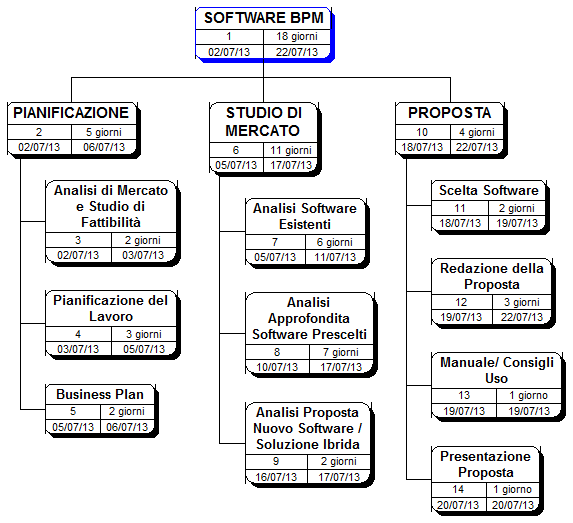
\includegraphics[width=\textwidth]{WBS}
	\caption{Work Breakdown Structure}
\end{figure}

\subsubsection{Pianificazione}
In questa fase verranno eseguite tutte le attività necessarie alla pianificazione del progetto.
Dovranno essere pianificate le attività da svolgere, i tempi e le risorse necessarie. Dovrà inoltre essere redatto il Business  Plan.
\paragraph{Analisi di Mercato e Studio di Fattibilità}



\begin{itemize}
\item{\bfseries Descrizione:}Questo WP prevede uno studio generale del mercato sui \inglese{software} BPM, con lo scopo di permettere l'organizzazione della pianificazione in base alle informazioni tratte dagli studi.
In particolare, lo studio di fattibilità dà al team la possibilità di capire se gli strumenti e le risorse di cui dispone sono sufficienti a garantire il conseguimento dell'obbiettivo.
L'analisi, invece, permetterà di eseguire una corretta pianificazione sulla base di informazioni vere riguardanti il mercato attuale. 
\item {\bfseries Responsabile:}
\item  {\bfseries Attività:}
	\begin{itemize}
		\item Ricerche in rete
		\item Analisi ad alto livello delle funzionalità dei \inglese{software} BPM
		\item Ricerche brevettuali
	\end{itemize}
\item  {\bfseries Costo:}
\item  {\bfseries Tempo di realizzazione: }2 giorni lavorativi
\end{itemize}



\paragraph{Pianificazione del Lavoro}
\begin{itemize}
\item{\bfseries Descrizione:} Questa attività prevede la pianificazione del lavoro in seguito allo studio di fattibilità effettuato. Il lavoro deve essere organizzato nelle sue attività e nei suoi tempi.
\item {\bfseries Responsabile:}
\item  {\bfseries Attività:}
	\begin{itemize}
		\item Stesura WBS
		\item Stesrua OBS
		\item Matrice delle responsabilità
		\item Stesrua RBS
		\item Diagramma di Gantt	
	\end{itemize}

\item  {\bfseries Costo:}
\item  {\bfseries Tempo di realizzazione:} 3 giorni lavorativi
\end{itemize}


\paragraph{Redazione Business Plan}
\begin{itemize}
\item{\bfseries Descrizione:} Questo WP prevede la redazione del Business Plan. Tale documento è molto importante sia a titolo organizzativo che rappresentativo, del progetto e dell'azienda stessa.
\item {\bfseries Responsabile:}
\item  {\bfseries Attività:}
\item  {\bfseries Costo:}
\item  {\bfseries Tempo di realizzazione:} 2 giorni lavorativi
\end{itemize}


\subsection{Studio di Mercato}
\paragraph{Studio dei Software Esistenti }
\begin{itemize}
\item{\bfseries Descrizione:} Questa attività prevede l'analisi dei \inglese{software} già presenti nel mercato. Si tratta di analizzare le diverse soluzioni già esistenti in commercio ed individuare quelle più adatte all'obbiettivo del progetto. 

\item {\bfseries Responsabile:}
\item  {\bfseries Attività:}
		\begin{itemize}
		\item Analisi generica del delle soluzioni \inglese{software} già presenti nel mercato
		\item Individuazione di una lista di \inglese{software} da visionare
		\item Analisi generale dei \inglese{software}
		\end{itemize}

\item  {\bfseries Costo:}
\item  {\bfseries Tempo di realizzazione:} 6 giorni lavorativi
\end{itemize}

\paragraph{Studio dei Software Prescelti}
\begin{itemize}
\item{\bfseries Descrizione:}  Questa attività prevede l'analisi dei \inglese{software} prescelti. Si tratta di analizzare e studiare e confrontare le prestazioni dei vari software. Le caratteristiche che si terranno in considerazione sono:

%TODO
\item {\bfseries Responsabile:}
\item  {\bfseries Attività:}
\begin{itemize}

		\item Individuazione della lista degli aspetti da tenere in considerazione
		\item Analisi individuale di ogni \inglese{software}
		\item Confronto dei diversi \inglese{software}
		\end{itemize}

\item  {\bfseries Costo:}
\item  {\bfseries Tempo di realizzazione:} 7 giorni lavorativi
\end{itemize}


\paragraph{Analisi Proposta Nuovo Software o Soluzione Ibrida }
\begin{itemize}
\item{\bfseries Descrizione:} Qusto WP prevede l'analisi della possibilità della realizzazione di un nuovo \inglese{software} o di una soluzione ibrida. Tale analisi avverrà soltanto dopo aver analizzato i diversi \inglese{software} prescelti e la scelta sarà scaturita dalla possibilità che nessun \inglese{software} attualmente in commercio soddisfi pienamente le richieste.
\item {\bfseries Responsabile:}
\item  {\bfseries Attività:}
\item  {\bfseries Costo:}
\item  {\bfseries Tempo di realizzazione:} 2 giorni lavorativi
\end{itemize}




\subsubsection{Proposta}


\paragraph{Scelta Software }
\begin{itemize}
\item{\bfseries Descrizione:} Questa attività è un punto cruciale. Da essa dipende il contenuto della proposta che sarà presentata. Si tratta di decidere il \inglese{software} BPM più adatto alle esigenze richieste.
\item {\bfseries Responsabile:}
\item  {\bfseries Attività:}
\item  {\bfseries Costo:}
\item  {\bfseries Tempo di realizzazione:} 2 giorni lavorativi
\end{itemize}

\paragraph{Redazione della Proposta }
\begin{itemize}
\item{\bfseries Descrizione:} Una volta che la scelta del \inglese{software} è avvenuta, sarà necessario presentarla in modo formale all'azienda richiedente. Si noti che la forma con cui presentiamo il lavoro svolto è fondamentale per avere successo e portare a termine gli obiettivi prefissati.
\item {\bfseries Responsabile:}
\item  {\bfseries Attività:}
	\begin{itemize}
	\item Individuazione del contenuto della proposta
	\item Stesura del documento
	\item Verifica del documento
 	\item Approvazione del documento	
	\end{itemize}

\item  {\bfseries Costo:}
\item  {\bfseries Tempo di realizzazione:} 2 giorni lavorativi
\end{itemize}


\paragraph{Redazione Manuale/Consigli d'uso}
\begin{itemize}
\item{\bfseries Descrizione:} Questo WP consiste nella redazione di un breve manuale per l'uso del \inglese{software} con il fine di facilitare gli utenti che ne faranno uso.
\item {\bfseries Responsabile:}
\item  {\bfseries Attività:}
	\begin{itemize}
	\item Individuazione del contenuto del manuale
	\item Scelta della forma di presentazione
	\item Verifica 
 	\item Approvazione	
	\end{itemize}

\item  {\bfseries Costo:}
\item  {\bfseries Tempo di realizzazione:}  1 giorno lavorativo
\end{itemize}

\paragraph{Presentazione Proposta}
\begin{itemize}
\item{\bfseries Descrizione:} Questo WP costituisce la conclusione di tutto il lavoro di progetto svolto. Si tratta di riassumere in una breve presentazione i contenuti del progetto e in particolari i motivi che hanno portato alla scelta di un determinato \inglese{software}.
\item {\bfseries Responsabile:}
\item  {\bfseries Attività:}
\begin{itemize}
	\item Individuazione del contenuto della presentazione
	\item Creazione della presentazione
	\end{itemize}


\item  {\bfseries Costo:}
\item  {\bfseries Tempo di realizzazione:}  1 giorno lavorativo
\end{itemize}




\section{Organizational Breakdown Structure}
l'Organizational Breakdown Structure (OBS) rappresenta l'organizzazione del progetto rispetto alle risorse umane impiegate in esso.
L'OBS rappresenta una scomposizione gerarchica delle responsabilità di progetto, generata alla scopo di individuare e responsabili dei WP. 
L'OBS deve essere creata in seguito alla redazione della WBS. Infatti, solo dopo aver tracciato i WP è possibile assegnare loro un responsabile/esecutore.
La creazione della OBS risulta utile sia sotto l'aspetto gerarchico in quanto permette al \inglese{Project Manger} di individuare i responsabili, sia sotto l'aspetto organizzativo degli esecutori materiali delle attività, in quanto facilita la comunicazione tra essi permettendo di capire a chi chiedere cosa. 

\clearpage
\begin{figure}[h!]
  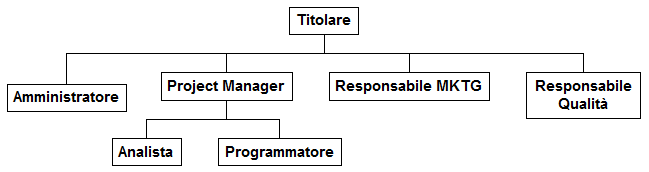
\includegraphics[width=\textwidth]{OBS}
	\caption{Organizational Breakdown Structure}
\end{figure}


Come si evince dal diagramma, tutti i responsabili sono a capo del titolare dell'azienda. Essendo infatti una piccola azienda il controllo, pure essendo distribuito rimane comunque sotto la supervisione del titolare.
Il Project Manager è invece a capo dell' Analista e del Programmatore. 
 
	\subsection{Titolare}
	È colui che possiede l'azienda (in tutto o in parte).
	\subsection{Amministratore}		
	L'amministratore è una figura molto importante dal punto di vista organizzativo. Ogni decisione deve essere approvata da 	tale figura e perciò deve essere messo al corrente di cosa succede sia nelle attività ordinarie che in quelle di progetto.
	Egli è responsabile dell'efficienza e dell'operatività dell'ambiente di sviluppo.Controlla inoltre versioni e configurazioni del prodotto.
	\subsection{Project Manager}
	Il Project Manager ha un ruolo determinante nella gestione dei progetti. Esso infatti è responsabile della valutazione, pianificazione, realizzazione e controllo di un progetto.
	I suoi compiti più importanti sono:
	\begin{itemize}
		\item Valutazione di costi e benefici del progetto
		\item Pianificazione del progetto
		\item Valutazione dello stato di avanzamento del progetto
		\item Pianificazione e gestione dei rischi di progetto
	\end{itemize}
	\subsection{Responsabile Marketing}
	Questo ruolo si occupa della definizione ed applicazione delle strategie di \inglese{marketing}. Egli si occupa delle relazioni con i clienti e della promozione delle attività dell'azienda stessa. Tale figura si occupa inoltre, del monitoraggio dei dati di mercato, degli indicatori e dei canali di vendita, al fine di permettere l'identificazione di nuove opportunità di \inglese{business}.
	Tale figura deve avere ottime capacità relazionali, manageriali e di \inglese{leadership}. 
\subsection{Responsabile Qualità}	
	La qualità è fondamentale per avere successo nei progetti. Oggi è una proprietà irrinunciabile, sia per clienti che fornitori. Per i clienti si tratta infatti di un'assicurazione sul prodotto/servizio che acquistano e per i fornitori, invece, costituisce  un punto di distinzione rispetto ai concorrenti.
Pur essendo una piccola azienda, si punta al raggiungimento della qualità, tramite l'adeguamento allo standard ISO/IEC 9001.
Nell'ambito dei progetti aziendali il Responsabile Marketing deve assicurare l'attuazione dei processi volti a garantire il rilascio di un prodotto/servizio che rispetta tutti i requisiti di qualità stabiliti.
	 
\subsection{Analista}
	L'analista ha un ruolo fondamentale nella fase iniziale del progetto. Tale figura deve infatti effettuare lo studio di fattibilità preoccupandosi dell'aspetto tecnico. In questo caso è molto importante perché dalla sua valutazione rispetto agli obiettivi del progetto, dipende in gran parte il successo o il fallimento del progetto.
\subsection{Programmatore}
	 Tale ruolo, in generale, dovrebbe semplicemente seguire le direttive di un Progettista per produrre il codice finale del prodotto. In questo casa, essendo l'azienda molto piccola ed il progetto particolare, egli avrà il compito di supportare l'analista nello studio di fattibilità e di analizzare i \inglese{software} secondo la sua esperienza.




\section{Matrice delle Responsabilità}
\section{Resource Breakdown Structure}
\section{Pianificazione Temporale}
\end{document}